\documentclass[border=1pt]{standalone}
\usepackage{tikz}
\usetikzlibrary{intersections, decorations.pathreplacing}


\begin{document}
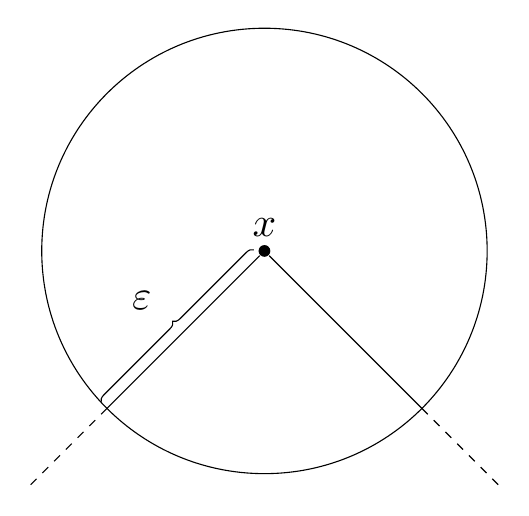
\begin{tikzpicture}[every node/.style={scale=1.5}]
  \node[fill=black, circle, inner sep=1pt] (x) at (0,0) {};
  \node[above] () at (x) {$x$};

  % Radius of the ball
  \pgfmathsetmacro{\r}{2*sqrt(2)}

  % Draw the circle
  \draw (x) circle (\r);

  % Use a 45-45-90 triangle for the edges
  \coordinate (side1end) at (-2, -2);
  \coordinate (side2end) at (2, -2);

  \draw (side1end) -- (x);
  \draw (side2end) -- (x);

  % Extend them past our epsilon ball with dotted segments
  \coordinate (side1ext) at (-3, -3);
  \coordinate (side2ext) at (3, -3);

  \draw[dashed] (side1end) -- (side1ext);
  \draw[dashed] (side2end) -- (side2ext);



  % Draw the label for \varepsilon with a brace
  \draw [
    decoration={
      brace,
      mirror,
      raise=3
    },
    decorate
  ] (x) -- (side1end) node[midway, yshift=.75em, xshift=-1em] {$\varepsilon$};



\end{tikzpicture}
\end{document}
